\chapter{Cores: the minimal structural information}\label{ch:minimal}

\Cref{thm:nerve} says that the dead-set pattern $D_A$ determines $\beta_2$. How much of $D_A$ must an observer see? This chapter measures, on the six-label census, how much \emph{count-level} information about the nerve (numbers of vertices, edges, triangles, Euler characteristics, numbers of hollow triangles) leaves uncertain about whether $\beta_2>0$, and contrasts it with a \emph{structural} reduction that preserves the answer exactly: strong collapse of the nerve to its core, followed by one $H_1$ computation. Counts are insufficient; the core is sufficient by a theorem; the core is not claimed to be minimal.

\section{Strong collapses and cores}
Let $\mathcal K$ be a finite simplicial complex. A vertex $v$ is \emph{dominated} by a vertex $w\neq v$ if every maximal simplex of $\mathcal K$ containing $v$ also contains $w$. Deleting a dominated vertex, together with all simplices containing it, is a \emph{strong collapse}; the result is a deformation retract of $\mathcal K$.
@@thm:barmak@@
@@cor:core-suffices+analytic@@

\section{What counts cannot see}\label{sec:D21}
Let $\mathcal P_{21}$ be the set of distinct rank-indexed dead-set patterns arising in the six-label census. The census has $346{,}859$ regimes, of which $8{,}008$ are fully admissible (there $Y_A=\emptyset$) and are excluded, leaving $338{,}851$ regimes with $219{,}145$ distinct patterns, $151$ of them with $\beta_2>0$ (carried by $158$ positive regimes). For each pattern the numbers of vertices, edges and triangles of the nerve, the Euler characteristic of its $2$-skeleton, the number of hollow triangles and the size of the strong-collapse core were computed.
\begin{table}[ht]\centering\small
\begin{tabular}{@{}lrrr@{}}\toprule
observation $O$ of the nerve & $H(Y|O)$ natural & $H(Y|O)$ balanced & classes\\ \midrule
$V=|D|$ & $0.0049$ & $0.5122$ & $57$\\
$(V,E)$ & $0.0037$ & $0.2418$ & $388$\\
Euler characteristic of the $2$-skeleton & $0.0020$ & $0.1073$ & $10{,}930$\\
number of hollow triangles & $0.0038$ & $0.1919$ & $2{,}639$\\
$(V,E,\#\text{triangles})$ & $0.0006$ & $0.0052$ & $20{,}595$\\
collapse-core size & $0.0009$ & $0.0319$ & $57$\\
(core size, hollow count) & $0.00002$ & $0.00007$ & $11{,}468$\\
collapse core, then $H_1$ & $0$ & $0$ & ---\\ \bottomrule
\end{tabular}
\caption{Exact residual uncertainty (bits) about $\beta_2>0$ over the six-label census for count-level observations of the dead-set nerve. The last row is a control: by \cref{cor:core-suffices} it computes $Y$ exactly. These values were obtained in the earlier companion computation and are not recomputed here (\cref{app:status}).}\label{tab:D21}
\end{table}
@@obs:collapse+finite-exact@@
\begin{figure}[ht]\centering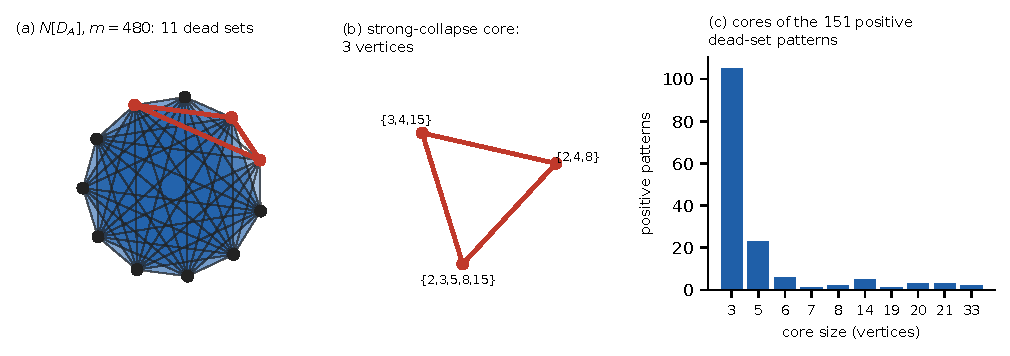
\includegraphics[width=\textwidth]{figures/fig_core.pdf}
\caption{(a)~The dead-set nerve of content $(2,3,4,5,8,15)$ at source $480$ ($11$ dead sets). (b)~Its strong-collapse core: three vertices forming the boundary of a triangle, so $\beta_2=1$. Both are drawn from the exact computation. (c)~Core sizes of the $151$ positive dead-set patterns of the census (recomputed exactly).}\label{fig:collapse}
\end{figure}
The question ``what is the minimal structural information that determines whether a hole exists?'' has three different answers depending on the observer. \emph{Without structure} (counts only), no tested statistic suffices (\cref{tab:D21}). \emph{With the dead-set pattern}, the answer is determined (\cref{thm:nerve}). \emph{With a homotopy-preserving reduction}, a hollow triangle in $105$ of the $151$ positive patterns is the entire information. No universal optimality is claimed: a smaller sufficient observation of the pattern could exist, and no lower bound is proved.
@@prop:counts-fail+finite-exact@@
A hollow triangle is a triple of forbidden prefix sets, pairwise compatible, with no prefix set related to all three. By \cref{obs:cycle-census} it occurs in $288$ of the $290$ positives and also in many negatives, where it always bounds. The difference between a bounding and a non-bounding hollow triangle is homological rather than local.
